\chapter{Query} 

\section{Query1}

\section{Query2}

\section{Query3}

\section{Query4}

\section{Query5}

\section{Query6}

\chapter{Trigger e Funzioni} 

\section{Trigger}

\subsection{InserimentoRetribuzione}
\lstinputlisting[language=SQL,firstline=98,lastline=110]{sql/DDL_Database.sql}

Il trigger esprime il vincolo semantico che la retribuzione di un'istruttore non possa essere un valore negativo (minore o uguale a zero). Nel caso lo sia, imposta una retribuzione base di 800 euro.
Questo trigger è dedicato alle operazioni di inserimento.

\subsection{AggiornaRetribuzione}
\lstinputlisting[language=SQL,firstline=112,lastline=124]{sql/DDL_Database.sql}

Trigger simile al precedente, utilizzato in caso di aggiornamento del campo retribuzione. Nel caso la retribuzione dell'istruttore venga impostata ad un valore negativo, viene ripristinato il vecchio valore.

Sono stati necessari due trigger visto che MySQL non permette di definire trigger su condizioni multiple.

\subsection{CorsoAttivoIns}
\lstinputlisting[language=SQL,firstline=126,lastline=137]{sql/DDL_Database.sql}

Imposta un corso come non attivo se manca il codice fiscale dell'istruttore che lo tiene. Vale per l'inserimento di nuovi corsi.

\subsection{CorsoAttivoUpd}

\lstinputlisting[language=SQL,firstline=139,lastline=150]{sql/DDL_Database.sql}

Imposta un corso come non attivo se manca il codice fiscale dell'istruttore che lo tiene. Vale per l'aggiornamento dei corsi.

\subsection{CorsoAttivoElim}

\lstinputlisting[language=SQL,firstline=152,lastline=166]{sql/DDL_Database.sql}

Come i trigger precedenti, si occupa di impostare il campo \textit{Attivo} di un corso a false (0) se viene eliminato l'istruttore che tiene quel corso.

\section{Funzioni}

\subsection{ControlloPrenotazione}

\lstinputlisting[language=SQL,firstline=173,lastline=193]{sql/DDL_Database.sql}

\subsection{ControlloPrenotazioneCorso}

\lstinputlisting[language=SQL,firstline=196,lastline=221]{sql/DDL_Database.sql}

\subsection{PossoIscrivermi}

\lstinputlisting[language=SQL,firstline=224,lastline=266]{sql/DDL_Database.sql}

\section{Schema concettuale E-R}
\begin{figure}[H]
 \centering
  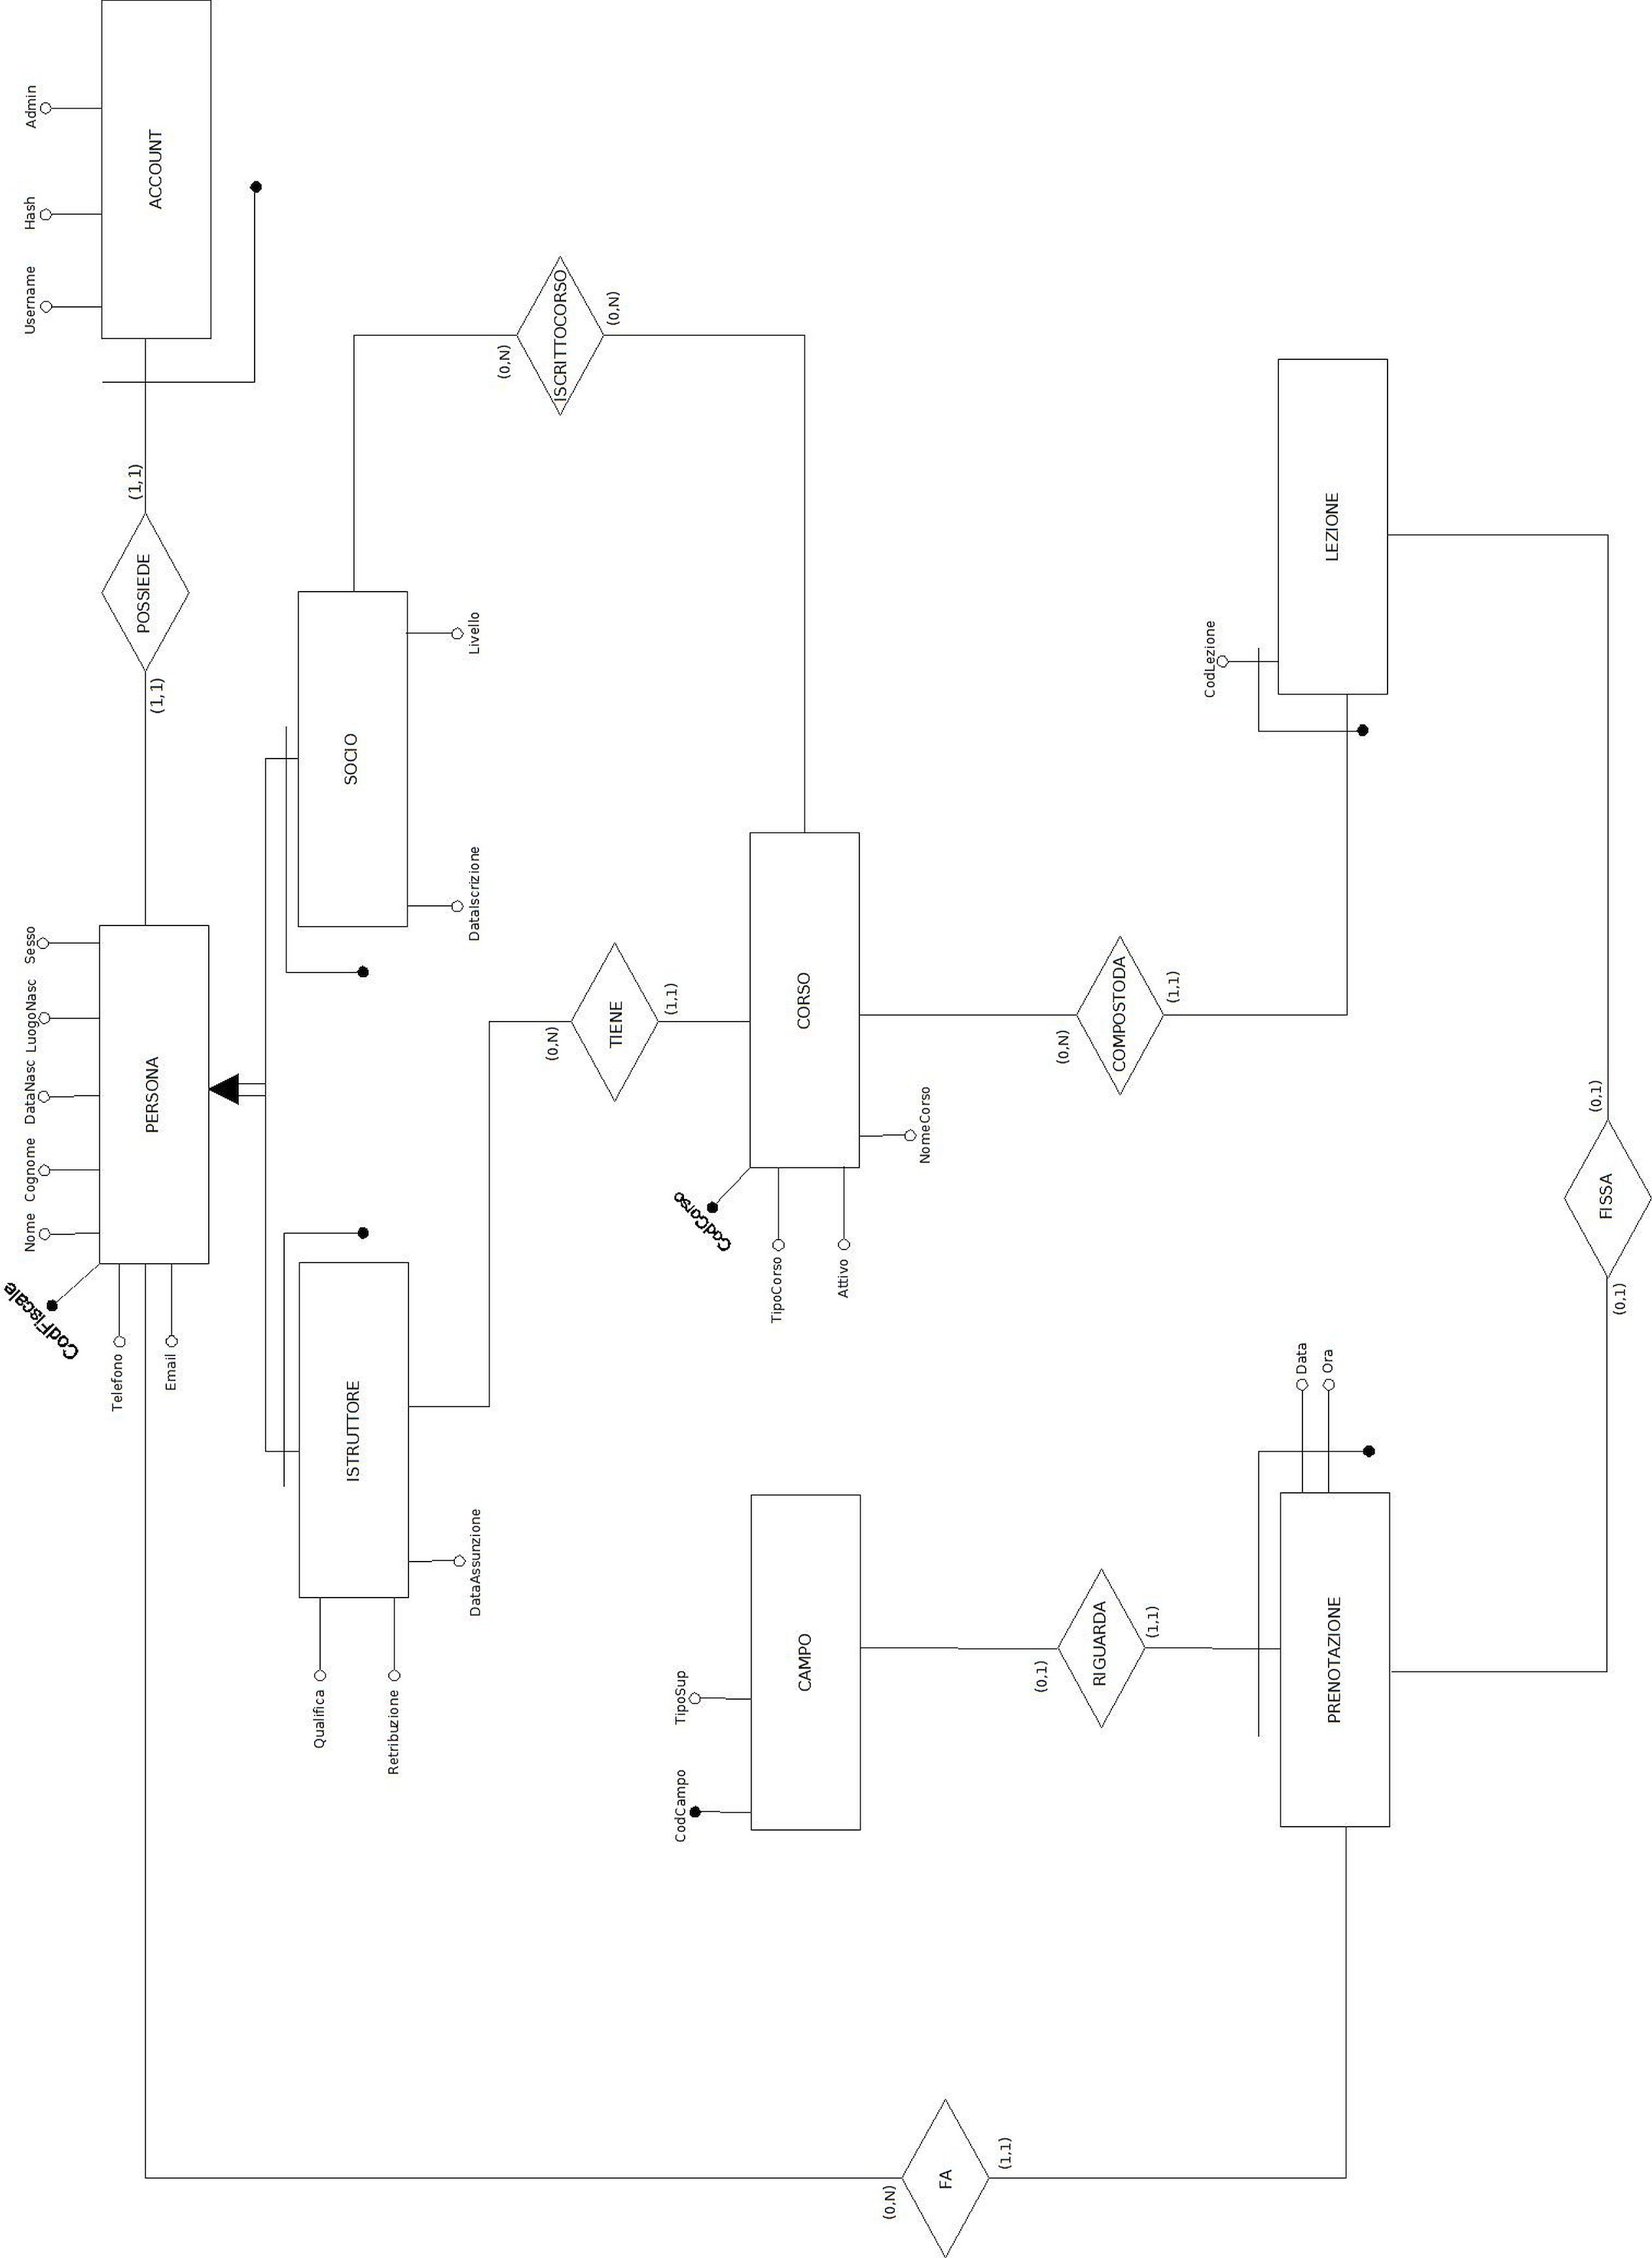
\includegraphics[width=\textwidth, height=\textheight]{Images/ER_FINALE.jpg}
\caption{Schema Concettuale E-R}
\end{figure}